\FloatBarrier
\section{Experiments in full text}
\label{app:fulltext}

This section holds the text of the long version of the paper for the experiments of
Section~\ref{sec:results}, with the figures and tables that were left out of the main text. Tables
and figures that are in the main text are not repeated.

\subsection{Five tasks with instructions: the certified switch}
\label{sec:fivefull}



\begin{figure}[t]
  \centering
  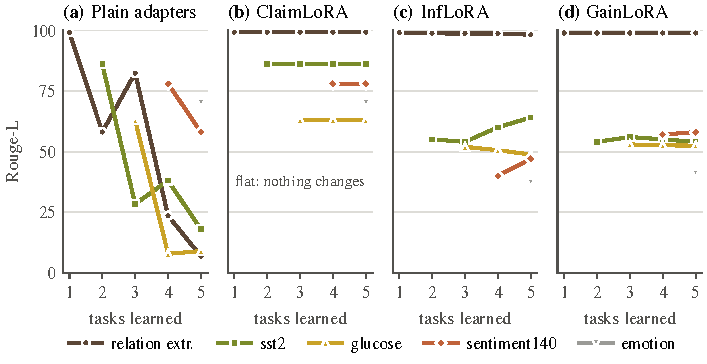
\includegraphics[width=\linewidth]{figures/five_tracks}
  \caption{Score of each of the five tasks as further tasks are learned (seed 42, original
  instructions). With plain adapters every task falls as soon as the next one is learned. With the
  certified switch the same adapters give flat lines. The two published methods are flat as well,
  at a lower level.}
  \label{fig:fivetracks}
\end{figure}

Table~\ref{tab:fivemain} and Figure~\ref{fig:fivetracks} give the result with instructions.

\paragraph{The certified switch keeps every answer.} With the certified switch the average score after the fifth task equals the
average score right after learning, \FiveCertAP{} Rouge-L. Forgetting is \FiveCertFT{}, and none of
the \FiveCertCompared{} answers to the test inputs of the first four tasks differs from the answer
that was given when the task had just been learned. All \FiveCertInputsOne{} test inputs lie inside
their own zone, as Proposition~\ref{prop:own} says they must, and no training input of a later
task lay inside an older zone (\FiveCertBlocked{} of \FiveCertTrainInputs{}). The outcome is therefore not an
observation about these runs but a consequence of Theorem~\ref{thm:writeonce}, and the experiment
confirms that the implementation does what the theorem describes. With the original instructions
\nearest{}, \centre{} and \keyswitch{} choose the same routes and give the same numbers.

\paragraph{The same adapters without a switch lose most of what they learned.} The rows from \cert{} to \plain{} use the same trained adapters; only the switches
differ. With all adapters on, the average falls from \FivePlainLearned{} right after learning to
\FivePlainAP{} at the end, forgetting is \FivePlainFT{} points, and \FivePlainChanged{} of
\FivePlainCompared{} answers change. Relation extraction, the first task, falls from
\FivePlainRelationLearned{} to \FivePlainRelationEnd{} on average over seeds (to 6.8 in the seed of
Figure~\ref{fig:fivetracks}a); only the task that was learned last is intact.

\paragraph{The published methods learned less here.} InfLoRA and GainLoRA have forgetting scores near zero in this setting
(\FiveInfFT{} and \FiveGainFT{} points; a
negative value means that old tasks improved on average while later ones were learned), though \FiveInfChanged{} and \FiveGainChanged{} of \FiveInfCompared{} answers change. Their curves
in Figure~\ref{fig:fivetracks} hardly fall. They nevertheless end at \FiveInfAP{}
and \FiveGainAP{}, well below the certified switch, because they are lower from the start: right
after learning, their tasks stand at \FiveInfLearned{} and \FiveGainLearned{} on average, against
\FiveCertLearned{} for plain adapters. Relation extraction is learned by both
(\FiveInfRelationLearned{} and \FiveGainRelationLearned{}). The classification tasks are not, within
ten epochs. On the two tasks with two labels the two methods are at the level of guessing right
after learning: \FiveInfSstLearned{} and \FiveGainSstLearned{} on SST-2 and
\FiveInfSentimentLearned{} and \FiveGainSentimentLearned{} on Sentiment140, where plain adapters
reach \FivePlainSstLearned{} and \FivePlainSentimentLearned{}; on emotion classification they stand
at \FiveInfEmotionLearned{} and \FiveGainEmotionLearned{} against \FivePlainEmotionLearned{}
(Table~\ref{tab:fivepertask} in the appendix). \textbf{So in our runs these two methods were at the level of guessing on two of the five tasks and clearly below plain adapters on a third, and the comparison cannot show how well they retain what they learn.} We do not know how much of this is the method and how much is our set-up: the budget is a
tenth of the published one, the model is smaller, and one step of both methods (a singular value
decomposition that the official code delegates to a library that did not load on the free GPUs) was
computed with PyTorch instead, without a check that the two agree number for number
(Appendix~\ref{app:impl}). A forgetting score at or
below zero also does not mean that nothing changes: \FiveInfChanged{} of \FiveInfCompared{} answers of
InfLoRA and \FiveGainChanged{} of \FiveGainCompared{} answers of GainLoRA are different at the end.
Changes for the better and for the worse cancel in the score.

\paragraph{The re-test agrees with the official test.} All numbers above come from the re-test, which scores every answer against all
reference answers. The scores written by the official script, which uses one randomly picked
reference per input, are \FiveCertOffAP{}, \FiveInfOffAP{} and \FiveGainOffAP{} for AP
(Table~\ref{tab:fiveofficial}) and lead to the same reading. With the original instructions the
re-test reproduced the answers of the official test on \FiveCertSame{} of \FiveCertSameOf{} inputs
for the certified switch, on \FiveInfSame{} of \FiveInfSameOf{} for InfLoRA and on \FiveGainSame{}
of \FiveGainSameOf{} for GainLoRA.

\paragraph{The same seed twice.} Seed 42 was run twice, in two separate sessions on the same kind
of GPU. For all three methods the first task was reproduced answer for answer (for the certified
switch and InfLoRA the second task as well), and the later tasks were not: for the certified
switch \RepeatCertSame{} of \RepeatCertTotal{} final
answers are the same, and the average score is \RepeatCertFirst{} in one run and
\RepeatCertSecond{} in the other (InfLoRA \RepeatInfFirst{} and \RepeatInfSecond{}, GainLoRA
\RepeatGainFirst{} and \RepeatGainSecond{}). Training is therefore not reproducible bit for bit on
this hardware, and differences of a few tenths of a point mean nothing. What does not vary is the
count for the certified switch: no answer of an earlier task changed in either run, nor in any
other seed. The tables use the second run of seed 42, which was made together with seeds 43
and 44.


\subsection{Reworded instructions}


\begin{figure}[t]
  \centering
  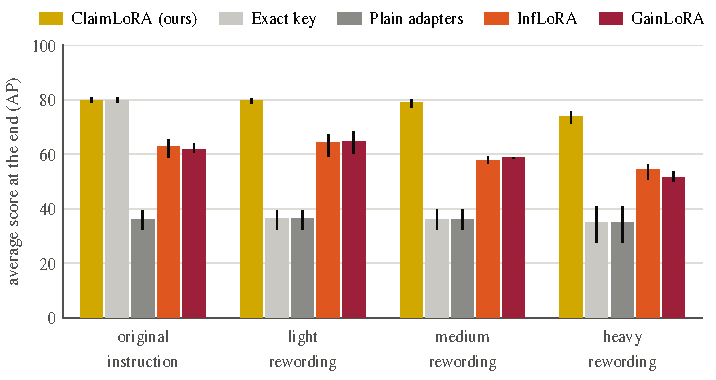
\includegraphics[width=0.9\linewidth]{figures/five_wordings}
  \caption{Average score at the end (AP) on the five tasks, with the original instructions and
  three levels of rewording. Bars are means over seeds; where there are several seeds a black line spans the lowest and the highest.}
  \label{fig:fivewordings}
\end{figure}

\begin{table}[t]
  \caption{Routes on the five tasks: how many test inputs are certified, how many are given to
  their own task, and how many answers change, for the certified switch and for the nearest-centre
  rule. Routes do not depend on the seed; counts are summed over seeds.}
  \label{tab:fiveroutes}
  \centering
  \small
  \setlength{\tabcolsep}{4.5pt}
  \begin{tabular}{lcccccc}
    \toprule
    & & \multicolumn{3}{c}{\cert{}} & \multicolumn{2}{c}{\centre{}} \\
    \cmidrule(lr){3-5} \cmidrule(lr){6-7}
    Wording & Tasks & Certified inputs & \shortstack[c]{Sent to own\\task $\uparrow$} & \shortstack[c]{Answers\\changed $\downarrow$} & \shortstack[c]{Sent to own\\task $\uparrow$} & \shortstack[c]{Answers\\changed $\downarrow$} \\
    \midrule
    original & 5 & 1{,}500 of 1{,}500 & 100.0\% & 0 of 1{,}200 & 100.0\% & 0 of 1{,}200 \\
    light & 5 & 1{,}500 of 1{,}500 & 100.0\% & 0 of 1{,}200 & 100.0\% & 0 of 1{,}200 \\
    medium & 5 & 300 of 1{,}500 & 100.0\% & 0 of 1{,}200 & 99.2\% & 0 of 1{,}200 \\
    heavy & 5 & 294 of 1{,}500 & 93.8\% & 0 of 1{,}200 & 72.2\% & 171 of 1{,}200 \\
    \bottomrule
\end{tabular}

\end{table}

\begin{table}[t]
  \caption{Five tasks, original and reworded: AP and changed answers (as Table~\ref{tab:fivemain}).}
  \label{tab:fivewordings}
  \centering
  \footnotesize
  \setlength{\tabcolsep}{3pt}
  \begin{tabular}{lcccccccc}
    \toprule
    & \multicolumn{4}{c}{Final score $\uparrow$} & \multicolumn{4}{c}{Answers changed (of 1{,}200) $\downarrow$} \\
    \cmidrule(lr){2-5} \cmidrule(lr){6-9}
    Method & original & light & medium & heavy & original & light & medium & heavy \\
    \midrule
    \cert{} (ours) & 79.7 & 79.6 & 79.0 & 74.1 & 0 & 0 & 0 & 0 \\
    \nearest{} & 79.7 & 79.6 & 79.0 & 74.1 & 0 & 0 & 0 & 0 \\
    \centre{} & 79.7 & 79.6 & 78.4 & 59.4 & 0 & 0 & 0 & 171 \\
    \keyswitch{} & 79.7 & 36.4 & 36.0 & 35.2 & 0 & 985 & 1{,}001 & 939 \\
    \plain{} & 36.1 & 36.4 & 36.0 & 35.2 & 994 & 985 & 1{,}001 & 939 \\
    \midrule
    InfLoRA & 62.9 & 64.3 & 57.8 & 54.3 & 370 & 296 & 320 & 470 \\
    GainLoRA & 62.0 & 64.6 & 58.8 & 51.6 & 65 & 58 & 122 & 178 \\
    \bottomrule
\end{tabular}

\end{table}


A benchmark input carries its task definition word for word, so any rule that recognises the
definition looks perfect. The test that separates the rules is to ask the same task in other
words. Table~\ref{tab:fivewordings} and Figure~\ref{fig:fivewordings} repeat the evaluation with the
three rewordings of each definition, and Table~\ref{tab:fiveroutes} shows where the inputs go.

\paragraph{No answer changes under any wording.} For the certified switch the number of changed answers is zero in every column.
With the light rewording this is again guaranteed, because all \FiveCertZoneOneLight{} inputs are
still certified (Table~\ref{tab:fiveroutes}). With the medium and the heavy rewording it is not
guaranteed: only \FiveCertZoneOneMedium{} and \FiveCertZoneOneHeavy{} of the \FiveCertInputsOne{}
inputs are inside a zone, and they belong to relation extraction, the task with the longest
instruction. The other inputs kept their answers because no later task came nearer to them than
the task they had been given to, which Proposition~\ref{prop:uncertified} permits but does not
promise. It also depends on the order of the tasks: in an order in which SST-2 is learned after
Sentiment140, 31 routes of heavily reworded inputs would change when SST-2 arrives
(Section~\ref{sec:orders}). The average
score falls from \FiveCertAP{} with the original instructions to \FiveCertAPLight{},
\FiveCertAPMedium{} and \FiveCertAPHeavy{}.

\paragraph{An exact key is a lookup table.} \keyswitch{} compares the opening token for token. With the original instructions
it is perfect. With the light rewording, which changes a few words, it recognises nothing, leaves
all adapters on and ends at \FiveKeyAPLight{}, exactly where \plain{} ends. It fails because an
input that it does not recognise gets every adapter. \nearest{} and \cert{} send such an input to
the nearest zone instead, and they score alike on this benchmark; the radius of the zones decides
which of these inputs also carry the guarantee.

\paragraph{The nearest centre of the whole input fails under heavy rewording.} \centre{}, the nearest-centre rule with the token weights of Eq.~\eqref{eq:weights}, gives only
\FiveCentreRightHeavy{}\% of the heavily reworded inputs to their own task. Its score is
\FiveCentreAPHeavy{} against \FiveCertAPHeavy{}, and \FiveCentreChangedHeavy{} of
\FiveCentreComparedHeavy{} answers change as later tasks arrive. The first version of our method, which used the nearest centre
with all tokens weighted equally, did better on these five tasks (97.4\% to the right task with seed 42, against
\FiveCertRightHeavy{}\% for the final rule) and was replaced because it failed on the 15-task sequence (Appendix~\ref{app:history}).

\paragraph{The published methods under rewording.} The published methods have no recognition step that a rewording could break, and
their forgetting scores stay within a few points in every wording, although many answers change (Table~\ref{tab:fivemore} in the
appendix). Their scores are \FiveInfAP{}, \FiveInfAPLight{}, \FiveInfAPMedium{} and
\FiveInfAPHeavy{} for InfLoRA and \FiveGainAP{}, \FiveGainAPLight{}, \FiveGainAPMedium{} and
\FiveGainAPHeavy{} for GainLoRA. The number of answers that differ at the end is largest under
heavy rewording, \FiveInfChangedHeavy{} and \FiveGainChangedHeavy{} of \FiveInfComparedHeavy{}.

\paragraph{Where the loss under heavy rewording comes from.} Under heavy rewording the certified switch scores \FiveCertAPHeavy{} instead of
\FiveCertAP{}. None of the difference is forgetting. One part is that the adapters themselves answer
a differently worded instruction less well: right after each task is learned, with all adapters on
(\plain{}), which at that moment is the right set of adapters, the score is
\FivePlainLearnedHeavy{}. The other part is routing:
\FiveCertWrongHeavy{} of the \FiveCertInputsOne{} heavily reworded inputs are given to another task,
which brings \FivePlainLearnedHeavy{} down to \FiveCertLearnedHeavy{}. All of them are tweets of the
Sentiment140 task that are given to SST-2, the other sentiment task.

\begin{figure}[t]
  \centering
  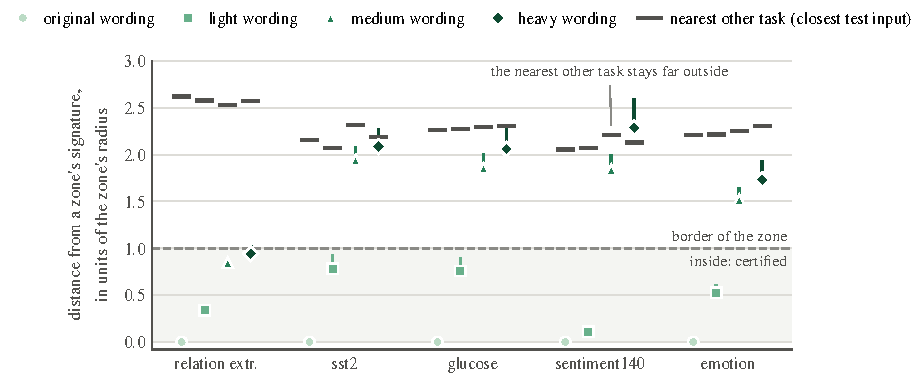
\includegraphics[width=0.92\linewidth]{figures/margins}
  \caption{Why rewording costs the certificate before it costs the route (five tasks, T5-base
  word-vectors). Markers: relative distance $\delta_k$ of the test inputs of a task from their own
  signature, in units of the radius of their own zone: median over the 100 inputs, with a line up to
  the farthest input. Short dark lines: how close the closest of these inputs comes to the signature of any
  \emph{other} task, in units of that task's radius. Below the dashed line an input is inside the
  zone, that is, certified.}
  \label{fig:margins}
\end{figure}

\paragraph{Where reworded inputs lie.}\label{sec:geometry} Figure~\ref{fig:margins} shows the geometry behind these numbers. With the original
wording every input lies exactly on the signature of its task (Proposition~\ref{prop:own}). The
light rewordings move the inputs by 0.1 to 0.8 radii, which is inside the zone. The medium and the
heavy rewordings move them by 1.5 to 2.3 radii in four of the five tasks, which is outside; relation
extraction, the task with the longest instruction, stays inside. The signatures of the other tasks,
however, are 2.1 to 2.6 of \emph{their} radii away from these inputs, so an input that has left its
zone is in most cases still nearer, in these units, to its own signature than to any other. The
certificate is lost long before the route is. The one place where the two margins cross is the
place of the errors: under the heavy rewording the tweets of Sentiment140 lie 2.29 radii from their
own signature (up to 2.60), and the signature of SST-2, the other sentiment task, is 2.13 of its
radii from the closest of them. Appendix~\ref{app:more} gives the numbers per task
(Table~\ref{tab:geometry}).

\subsection{Routes from the example alone: rewording cannot change the route}
\label{sec:exampleroutes}

The zones read the instruction, and a reworded instruction can leave them: under the heavy
rewording \cert{} sends some inputs to another task and ends below what the same adapters give
when every input reaches its own task (Section~\ref{sec:reworded}). \recog{} never
reads the instruction (Remark~\ref{rem:auditlimits}(v)). So the five tasks were trained once more
with their definitions (seed 42, plain adapters, nothing blocked), and the routes of \recog{} and
\handicap{} were computed from the example alone. It is the same route table as in the runs without
instructions (Section~\ref{sec:nodeftrained}), because these routes do not depend on the definition.
The scores of \cert{} in this run equal those of the earlier run of this seed at every wording.
Line fixed before the run: \recog{} ``repairs the weak spot'' if its final score at the heavy
wording is at least 2 points above that of \cert{}, its score at the original wording is within
2 points of \cert{}, and at most 8 of the \AudUCompared{} compared answers change at every wording;
it ``does not'' if the heavy score is below that of \cert{} or the original score more than 4
points below.

\begin{table}[t]
  \caption{The five tasks with their definitions, seed 42, T5-base, 10 epochs, plain adapters; the
  same adapters under each rule, at the four wordings of the definition. Top: final score (AP,
  re-test). Bottom: answers to the test inputs of the first four tasks that differ at the end from
  the answer right after their task was learned, of \AudUCompared{}. \recog{} and \handicap{} set
  the route from the example alone; ``zone first'' uses the certified route where the input is
  inside a zone and the route of \recog{} or \handicap{} elsewhere. The rows of the published
  methods are from the run of the same seed in Section~\ref{sec:reworded}.}
  \label{tab:instanceroutes}
  \centering
  {\scriptsize\setlength{\tabcolsep}{2pt}\begin{tabular}{p{1.2in}rrrrrrrrr}
    \toprule
    & \multicolumn{4}{c}{Final score $\uparrow$} & \multicolumn{4}{c}{\shortstack{Answers changed\\of \AudUCompared{} $\downarrow$}} & \shortstack[r]{Sent to own\\task, heavy, \% $\uparrow$} \\
    \cmidrule(lr){2-5}\cmidrule(lr){6-9}
    & original & light & medium & heavy & original & light & medium & heavy & \\
    \midrule
    \cert{} (zones on the instruction) & \AudUOriginalCertAP{} & \AudULightCertAP{} & \AudUMediumCertAP{} & \AudUHeavyCertAP{} & \AudUOriginalCertChanged{} & \AudULightCertChanged{} & \AudUMediumCertChanged{} & \AudUHeavyCertChanged{} & \AudUHeavyCertRight{} \\
    \recog{} (example alone) & \AudUOriginalRidgeAP{} & \AudULightRidgeAP{} & \AudUMediumRidgeAP{} & \AudUHeavyRidgeAP{} & \AudUOriginalRidgeChanged{} & \AudULightRidgeChanged{} & \AudUMediumRidgeChanged{} & \AudUHeavyRidgeChanged{} & \AudUHeavyRidgeRight{} \\
    \handicap{}, $\nu = 2$ (example alone) & \AudUOriginalHandicapAP{} & \AudULightHandicapAP{} & \AudUMediumHandicapAP{} & \AudUHeavyHandicapAP{} & \AudUOriginalHandicapChanged{} & \AudULightHandicapChanged{} & \AudUMediumHandicapChanged{} & \AudUHeavyHandicapChanged{} & \AudUHeavyHandicapRight{} \\
    every input to its own task (ceiling) & \AudUOriginalOwnAP{} & \AudULightOwnAP{} & \AudUMediumOwnAP{} & \AudUHeavyOwnAP{} & \AudUOriginalOwnChanged{} & \AudULightOwnChanged{} & \AudUMediumOwnChanged{} & \AudUHeavyOwnChanged{} & \AudUHeavyOwnRight{} \\
    zone first, else \recog{} & \AudUOriginalMixRidgeAP{} & \AudULightMixRidgeAP{} & \AudUMediumMixRidgeAP{} & \AudUHeavyMixRidgeAP{} & \AudUOriginalMixRidgeChanged{} & \AudULightMixRidgeChanged{} & \AudUMediumMixRidgeChanged{} & \AudUHeavyMixRidgeChanged{} & \AudUHeavyMixRidgeRight{} \\
    zone first, else \handicap{} & \AudUOriginalMixHandicapAP{} & \AudULightMixHandicapAP{} & \AudUMediumMixHandicapAP{} & \AudUHeavyMixHandicapAP{} & \AudUOriginalMixHandicapChanged{} & \AudULightMixHandicapChanged{} & \AudUMediumMixHandicapChanged{} & \AudUHeavyMixHandicapChanged{} & \AudUHeavyMixHandicapRight{} \\
    \centre{} & \AudUOriginalCentreAP{} & \AudULightCentreAP{} & \AudUMediumCentreAP{} & \AudUHeavyCentreAP{} & \AudUOriginalCentreChanged{} & \AudULightCentreChanged{} & \AudUMediumCentreChanged{} & \AudUHeavyCentreChanged{} & \AudUHeavyCentreRight{} \\
    \plain{} & \AudUOriginalPlainAP{} & \AudULightPlainAP{} & \AudUMediumPlainAP{} & \AudUHeavyPlainAP{} & \AudUOriginalPlainChanged{} & \AudULightPlainChanged{} & \AudUMediumPlainChanged{} & \AudUHeavyPlainChanged{} & \AudUHeavyPlainRight{} \\
    \midrule
    GainLoRA & \AudWordOriginalGainloraAP{} & \AudWordLightGainloraAP{} & \AudWordMediumGainloraAP{} & \AudWordHeavyGainloraAP{} & \AudWordOriginalGainloraChanged{} & \AudWordLightGainloraChanged{} & \AudWordMediumGainloraChanged{} & \AudWordHeavyGainloraChanged{} & -- \\
    InfLoRA & \AudWordOriginalInfloraAP{} & \AudWordLightInfloraAP{} & \AudWordMediumInfloraAP{} & \AudWordHeavyInfloraAP{} & \AudWordOriginalInfloraChanged{} & \AudWordLightInfloraChanged{} & \AudWordMediumInfloraChanged{} & \AudWordHeavyInfloraChanged{} & -- \\
    \bottomrule
\end{tabular}}

\end{table}

Table~\ref{tab:instanceroutes} gives the result. At the heavy wording \recog{} ends at
\AudUHeavyRidgeAP{} and \handicap{} at \AudUHeavyHandicapAP{}, against \AudUHeavyCertAP{} for
\cert{} (seed 42; the mean over three seeds in Section~\ref{sec:reworded} is \FiveCertAPHeavy{});
the ceiling, with every input at its own task, is \AudUHeavyOwnAP{}. At the original
wording \recog{} ends at \AudUOriginalRidgeAP{} and \handicap{} at \AudUOriginalHandicapAP{},
against \AudUOriginalCertAP{}. At every wording \AudUOriginalRidgeChanged{} of \AudUCompared{}
answers change under \recog{} and \AudUOriginalHandicapChanged{} under \handicap{}, where \cert{}
changes none. All three lines hold: the verdict is ``repairs the weak spot''.
Our guesses (78.5 to 79.3 at the original wording, 75.5 to 76.7 at the heavy one) held, and one
was wrong in the good direction: we had expected about six changed answers for \recog{}, as in
the run without definitions. Six routes do change, but for three
of these inputs the model gives the same answer with the adapters up to either task. Without
definitions all six answers changed; why fewer change with the definition we did not test.

What this shows: the routes of \recog{} are the same at every wording, so its score stays
\AudURidgeBelowOwnLow{} to \AudURidgeBelowOwnHigh{} points below the ceiling at every wording
(\handicap{}: \AudUHandicapBelowOwnLow{} to \AudUHandicapBelowOwnHigh{} points), and what is lost
under rewording is what the adapters themselves lose when their instruction is reworded, not
misrouting. The zones are exact where the instruction is unedited and lose
\AudUHeavyCertBelowOwn{} points at the heavy wording through misrouted
inputs. The mixed rule has the best of both at the original, the light and the heavy wording; at
the medium wording it is below \cert{} (\AudUMediumMixRidgeAP{} and \AudUMediumMixHandicapAP{}
against \AudUMediumCertAP{}), whose own fallback is right for every input there. The published
methods end at \AudWordHeavyGainloraAP{} (GainLoRA) and \AudWordHeavyInfloraAP{} (InfLoRA) at the
heavy wording, with \AudWordHeavyGainloraChanged{} and \AudWordHeavyInfloraChanged{} changed
answers. This first run is one seed, five tasks, and three machine-written rewordings per task
that were looked at during development (Section~\ref{sec:protocol}), not
rewordings by people. Remark~\ref{rem:auditlimits}(v) says what this assumes about
the input.

\paragraph{Three seeds.} An independent reading of this result pointed out that seed 42 is the seed in which \cert{} loses most at the heavy wording. So the run was repeated for seeds 43 and 44 (Table~\ref{tab:instanceroutesseeds}).
Line fixed before these runs, for the means over the three seeds: the result ``stands for three seeds'' if the heavy score of \recog{} is at least 2 points above that of \cert{}, the original score is within 2 points of \cert{}, and in every seed at most 8 of \AudUCompared{} answers change at every wording.
It stands. At the heavy wording \recog{} ends at \AudUThreeHeavyRidgeAP{} and \handicap{} at \AudUThreeHeavyHandicapAP{}, against \AudUThreeHeavyCertAP{} for \cert{}, a gain of \AudUThreeHeavyRidgeAboveCert{} points; the ceiling is \AudUThreeHeavyOwnAP{}.
At the original wording \recog{} ends at \AudUThreeOriginalRidgeAP{}, \AudUThreeOriginalRidgeBelowCert{} points below \cert{} (\AudUThreeOriginalCertAP{}).
In no seed and at no wording do more than \AudUThreeMaxChangedPerSeed{} of \AudUCompared{} answers change under \recog{}.
Over the four wordings \recog{} stays \AudUThreeRidgeBelowOwnLow{} to \AudUThreeRidgeBelowOwnHigh{} points below the ceiling and \handicap{} \AudUThreeHandicapBelowOwnLow{} to \AudUThreeHandicapBelowOwnHigh{}; \cert{} loses \AudUThreeHeavyCertBelowOwn{} points at the heavy wording through misrouted inputs.
We had expected a smaller gain, 2 to 2.5 points: in seeds 43 and 44 the adapters themselves lose less under the heavy rewording than in seed 42.
It remains five tasks, with machine-written rewordings that were looked at during development.

\begin{table}[t]
  \caption{As Table~\ref{tab:instanceroutes}, means over \AudUThreeSeeds{} seeds (42, 43, 44); changed answers are summed over the seeds.}
  \label{tab:instanceroutesseeds}
  \centering
  {\scriptsize\setlength{\tabcolsep}{2pt}\begin{tabular}{p{1.2in}rrrrrrrrr}
    \toprule
    & \multicolumn{4}{c}{Final score $\uparrow$} & \multicolumn{4}{c}{\shortstack{Answers changed\\of \AudUThreeCompared{} $\downarrow$}} & \shortstack[r]{Sent to own\\task, heavy, \% $\uparrow$} \\
    \cmidrule(lr){2-5}\cmidrule(lr){6-9}
    & original & light & medium & heavy & original & light & medium & heavy & \\
    \midrule
    \cert{} (zones on the instruction) & \AudUThreeOriginalCertAP{} & \AudUThreeLightCertAP{} & \AudUThreeMediumCertAP{} & \AudUThreeHeavyCertAP{} & \AudUThreeOriginalCertChanged{} & \AudUThreeLightCertChanged{} & \AudUThreeMediumCertChanged{} & \AudUThreeHeavyCertChanged{} & \AudUThreeHeavyCertRight{} \\
    \recog{} (example alone) & \AudUThreeOriginalRidgeAP{} & \AudUThreeLightRidgeAP{} & \AudUThreeMediumRidgeAP{} & \AudUThreeHeavyRidgeAP{} & \AudUThreeOriginalRidgeChanged{} & \AudUThreeLightRidgeChanged{} & \AudUThreeMediumRidgeChanged{} & \AudUThreeHeavyRidgeChanged{} & \AudUThreeHeavyRidgeRight{} \\
    \handicap{}, $\nu = 2$ (example alone) & \AudUThreeOriginalHandicapAP{} & \AudUThreeLightHandicapAP{} & \AudUThreeMediumHandicapAP{} & \AudUThreeHeavyHandicapAP{} & \AudUThreeOriginalHandicapChanged{} & \AudUThreeLightHandicapChanged{} & \AudUThreeMediumHandicapChanged{} & \AudUThreeHeavyHandicapChanged{} & \AudUThreeHeavyHandicapRight{} \\
    every input to its own task (ceiling) & \AudUThreeOriginalOwnAP{} & \AudUThreeLightOwnAP{} & \AudUThreeMediumOwnAP{} & \AudUThreeHeavyOwnAP{} & \AudUThreeOriginalOwnChanged{} & \AudUThreeLightOwnChanged{} & \AudUThreeMediumOwnChanged{} & \AudUThreeHeavyOwnChanged{} & \AudUThreeHeavyOwnRight{} \\
    zone first, else \recog{} & \AudUThreeOriginalMixRidgeAP{} & \AudUThreeLightMixRidgeAP{} & \AudUThreeMediumMixRidgeAP{} & \AudUThreeHeavyMixRidgeAP{} & \AudUThreeOriginalMixRidgeChanged{} & \AudUThreeLightMixRidgeChanged{} & \AudUThreeMediumMixRidgeChanged{} & \AudUThreeHeavyMixRidgeChanged{} & \AudUThreeHeavyMixRidgeRight{} \\
    zone first, else \handicap{} & \AudUThreeOriginalMixHandicapAP{} & \AudUThreeLightMixHandicapAP{} & \AudUThreeMediumMixHandicapAP{} & \AudUThreeHeavyMixHandicapAP{} & \AudUThreeOriginalMixHandicapChanged{} & \AudUThreeLightMixHandicapChanged{} & \AudUThreeMediumMixHandicapChanged{} & \AudUThreeHeavyMixHandicapChanged{} & \AudUThreeHeavyMixHandicapRight{} \\
    \centre{} & \AudUThreeOriginalCentreAP{} & \AudUThreeLightCentreAP{} & \AudUThreeMediumCentreAP{} & \AudUThreeHeavyCentreAP{} & \AudUThreeOriginalCentreChanged{} & \AudUThreeLightCentreChanged{} & \AudUThreeMediumCentreChanged{} & \AudUThreeHeavyCentreChanged{} & \AudUThreeHeavyCentreRight{} \\
    \plain{} & \AudUThreeOriginalPlainAP{} & \AudUThreeLightPlainAP{} & \AudUThreeMediumPlainAP{} & \AudUThreeHeavyPlainAP{} & \AudUThreeOriginalPlainChanged{} & \AudUThreeLightPlainChanged{} & \AudUThreeMediumPlainChanged{} & \AudUThreeHeavyPlainChanged{} & \AudUThreeHeavyPlainRight{} \\
    \midrule
    GainLoRA & \AudUThreeOriginalGainloraAP{} & \AudUThreeLightGainloraAP{} & \AudUThreeMediumGainloraAP{} & \AudUThreeHeavyGainloraAP{} & \AudUThreeOriginalGainloraChanged{} & \AudUThreeLightGainloraChanged{} & \AudUThreeMediumGainloraChanged{} & \AudUThreeHeavyGainloraChanged{} & -- \\
    InfLoRA & \AudUThreeOriginalInfloraAP{} & \AudUThreeLightInfloraAP{} & \AudUThreeMediumInfloraAP{} & \AudUThreeHeavyInfloraAP{} & \AudUThreeOriginalInfloraChanged{} & \AudUThreeLightInfloraChanged{} & \AudUThreeMediumInfloraChanged{} & \AudUThreeHeavyInfloraChanged{} & -- \\
    \bottomrule
\end{tabular}}

\end{table}


\subsection{Where the gap to the published methods comes from}
\label{sec:gap}

\begin{figure}[t]
  \centering
  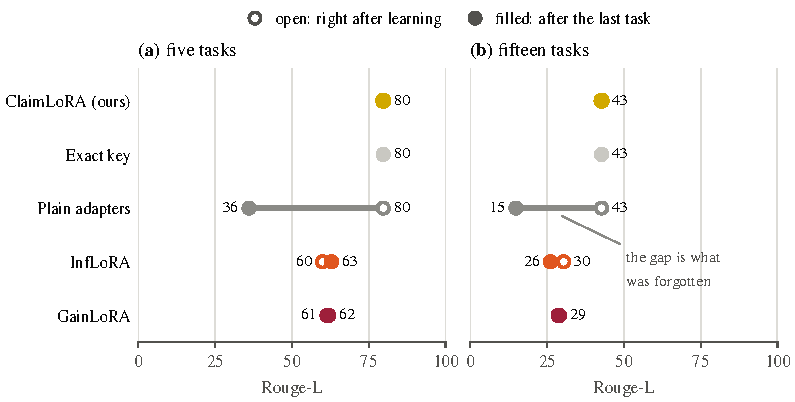
\includegraphics[width=0.9\linewidth]{figures/learn_forget}
  \caption{Learning and forgetting side by side, (a) on five tasks (mean over three seeds) and (b)
  on fifteen tasks (one seed). Open circle: average score of each task right
  after it was learned. Filled circle: average score after the last task. A gap between the two circles
  of a method is forgetting; an open circle far to the left is a lack of learning.}
  \label{fig:learnforget}
\end{figure}

Figure~\ref{fig:learnforget} separates the two things that a final score mixes.
For plain adapters the open circle is high and the filled circle is low: they learn and then forget.
For the two published methods on five tasks both circles are low and nearly equal: their forgetting scores are
near zero, but within ten epochs they have learned less. On fifteen tasks (panel b) their open circles are low
as well, and the filled circles are lower than the open ones for InfLoRA (\FifteenInfLearned{} to
\FifteenInfAP{}) and, by less, for GainLoRA (\FifteenGainLearned{} to \FifteenGainAP{}). The
certified switch has the open circle of plain adapters and no gap. On five tasks the comparison
therefore does not show that the published methods forget, and we do not claim that it does. On
fifteen tasks it shows some forgetting, and a larger lack of learning. In both, in our
set-up they had learned less by the time the next task arrived, for reasons we did not
separate (the method, the short budget, or our set-up), while the switch leaves the training of an
adapter untouched. The published results of both methods were
obtained with 100 epochs and T5-large. We could not run that setting, and the gap in learning may
well close there. Without instructions the same two methods did forget more
(Section~\ref{sec:nodefpublished}), with the same caveat on learning.




\subsection{What the zones add: a later task that looks like an old one}

On the benchmark sequences \nearest{} and \cert{} give the same routes, so the experiments above
cannot show what the frozen zones and the priority of older tasks are for. They matter when a later
task resembles an earlier one. We construct this case from the five-task sequence, at the level of
routes, which needs no GPU: after the five tasks a sixth task arrives whose inputs are of the same
kind as those of task~2 (SST-2 sentences) and whose definition is one of the rewordings of task~2's
definition. This is what happens when someone adds ``the same task again'' with a slightly
different instruction and possibly different labels. Table~\ref{tab:stress} counts how many of the
100 old test inputs of task~2, under each wording, are routed differently after the sixth task has
been added.

\begin{table}[t]
  \caption{Stress test (routes only). A sixth task with SST-2 inputs and a reworded SST-2 definition
  follows the five tasks. ``Blocked'': its training inputs inside an older zone. ``Routes changed'':
  old test inputs of task~2 (100 per wording) routed elsewhere afterwards.}
  \label{tab:stress}
  \centering
  \footnotesize
  \setlength{\tabcolsep}{3pt}
  \begin{tabular}{lccccccccc}
    \toprule
    & & \multicolumn{4}{c}{Routes changed, \cert{} $\downarrow$} & \multicolumn{4}{c}{Routes changed, \nearest{} $\downarrow$} \\
    \cmidrule(lr){3-6} \cmidrule(lr){7-10}
    New task's definition & Blocked & original & light & medium & heavy & original & light & medium & heavy \\
    \midrule
    light & 799 of 800 & 0 & 0 & 0 & 0 & 0 & 100 & 0 & 0 \\
    medium & 0 of 800 & 0 & 0 & 100 & 2 & 0 & 0 & 100 & 2 \\
    heavy & 0 of 800 & 0 & 0 & 0 & 100 & 0 & 0 & 0 & 100 \\
    \bottomrule
\end{tabular}

\end{table}


\paragraph{A look-alike inside an old zone is blocked and reported.} If the definition of the new
task is the light rewording of task~2's definition, its inputs fall inside the zone of task~2: 799 of
its 800 training inputs are blocked. The user is told so when the task arrives, before any
training. Under \cert{} not a single old input changes its route. Under \nearest{} the picture is
different: the old inputs with the light rewording, which task~2 has answered until now, carry the
instruction of the new task word for word and lie exactly on its signature, and all 100 are
re-routed to it. The same text gets a different answer from then on, and nothing announces it.
This is the case the frozen zones exist for: under a rule that always picks the best match, the
arrival of a task can change answers that were given before; under the oldest-claim rule it
cannot, for a certified input. Section~\ref{sec:paraphrase} counts how often this occurs among \WidenTasksEval{} real tasks with machine-paraphrased instructions: rarely, and the zones did not prevent it there (\nearest{} and \cert{} changed the same \RerouteNearNChanged{} of \RerouteInputs{} routes), so this constructed case is not typical of that collection. Whether the old or the new task ought to answer such a text is a question the rules do not
settle. The test is one constructed case and it is about routes; no adapter was trained for the
sixth task.

\paragraph{A look-alike outside every zone can take uncertified inputs.} If the new definition is
the medium or the heavy rewording, the new signature lies outside the zone of task~2. Nothing is
blocked, the new task gets a zone of its own, and under both rules the old inputs that carry exactly
that rewording are re-routed (100 of 100, plus 2 inputs with the heavy wording in the medium case).
Those inputs were never certified. The certified inputs of task~2, the original and the light
wording, keep their route in every case. The stress test thus shows both sides of the guarantee:
it protects exactly the certified inputs, and it does not protect the others.


\subsection{What the zones cost: 875 real tasks}

The stress test built one look-alike task by hand. A large collection of real tasks contains
look-alikes by itself, and it shows how often the price of the guarantee has to be paid. We take
the \ManyTasks{} tasks of the default English split of Super-NaturalInstructions
\citep{wang2022superni}, each with its definition and its first inputs (\ManyInputs{} inputs;
openings of \ManyOpeningMin{} to \ManyOpeningMax{} tokens, \ManyOpeningMedian{} in the middle; the longest, \ManyOpeningMax{}, is the truncation length, so for these tasks the instance is cut off), let
them arrive in a random order, and give each task its zone when it arrives. No model is trained;
the test is about routes. Its rules, including what would count against the method, were fixed
before it was run (Appendix~\ref{app:many}).

\begin{table}[t]
  \caption{The zones on \ManyTasks{} real tasks in random order (routes only, unedited instructions).
  ``Blocked'': tasks with none, some or all inputs inside an older zone on arrival. ``Routes changed
  later'': inputs routed differently than on arrival, under \cert{} / \exactfirst{} / \nearest{}.}
  \label{tab:many}
  \centering
  \footnotesize
  \setlength{\tabcolsep}{3pt}
  \begin{tabular}{rccccccc}
    \toprule
    & \multicolumn{3}{c}{Tasks with blocked inputs} & \multicolumn{3}{c}{Inputs to their own task, \%} & Routes \\
    \cmidrule(lr){2-4} \cmidrule(lr){5-7}
    Tasks & none & some & all & \cert{} & \exactfirst{} & \nearest{} & changed later \\
    \midrule
    50 & 49 & 1 & 0 & 98.7 & 100.0 & 100.0 & 0 / 0 / 0 \\
    100 & 96 & 3 & 1 & 96.7 & 100.0 & 100.0 & 0 / 0 / 0 \\
    200 & 178 & 7 & 15 & 90.4 & 99.0 & 98.5 & 0 / 0 / 0 \\
    400 & 337 & 13 & 50 & 85.7 & 99.2 & 99.0 & 0 / 0 / 0 \\
    875 & 724 & 22 & 129 & 83.8 & 98.4 & 98.3 & 0 / 0 / 0 \\
    \bottomrule
\end{tabular}

\end{table}

\begin{figure}[t]
  \centering
  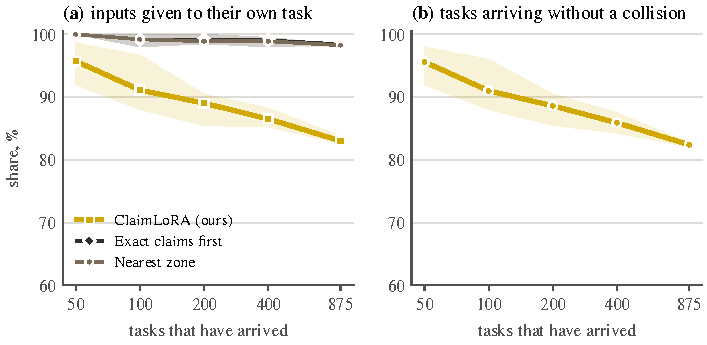
\includegraphics[width=0.86\linewidth]{figures/many}
  \caption{The price of the guarantee as the collection grows (same test as
  Table~\ref{tab:many}; lines are means over five random orders of arrival, bands span the lowest
  and the highest). (a) Share of inputs that are given to their own task; the variant of
  Section~\ref{sec:exactfirst} and the nearest-zone rule nearly coincide. (b) Share of tasks that
  arrive with no input inside an older zone.}
  \label{fig:many}
\end{figure}

\paragraph{The guarantee holds, and its price grows with the collection.} No certified input changed
its route, in any order of arrival and at any size of the collection. But the larger the
collection, the more often a new task arrives inside an older zone (Table~\ref{tab:many},
Figure~\ref{fig:many}). After all \ManyTasks{} tasks, \ManyColliding{} of them
(\ManyCollidingPct{}\%) have collided with an older task, and for \ManyAllHeld{} every input is
blocked, so that under their given instruction they could not be learned at all. In four other
random orders between \ManyCollidingPctLow{}\% and \ManyCollidingPctHigh{}\% of the tasks collide,
and in the order of the task numbers \ManyNumericCollidingPct{}\%. These collisions are not
accidents of the geometry. Of the \ManyColliding{} colliding tasks, \ManySameText{} have the same
definition text as the task they collide with, a further \ManyAlikeHigh{} share at least 80\% of its words,
and none shares less than \ManyAlikeLowest{}\%. They come from families
of tasks whose definitions differ in a word or two: \ManyFamilyMmlu{} are subject variants of one
multiple-choice task and \ManyFamilyAtomic{} are relation variants of one classification task
(examples in Table~\ref{tab:manyexamples}).

\paragraph{On unedited instructions the nearest-zone rule is the better rule.} \nearest{} gives
\ManyNearRightPct{}\% of the inputs to their own task and \cert{} \ManyCertRightPct{}\%, and under
neither rule is a single input re-routed after its task has arrived. The reason is simple. An
input with an unedited instruction lies exactly on the signature of its task, so no other zone can
be nearer, whatever arrives later. Before the test we had written down that we expected \nearest{}
to re-route inputs here; that was wrong. The weakness of \nearest{} needs edited inputs, as in
Section~\ref{sec:stress}, and the unedited inputs of this collection contain none. Section~\ref{sec:paraphrase} adds machine paraphrases to the collection and
counts the re-routing: \nearest{} changed \RerouteNearNChanged{} of \RerouteInputs{} routes there, the same as \cert{}.

\paragraph{The trade, stated plainly.} A zone protects a neighbourhood of an old instruction, where its light rewordings and fewer than half of its machine paraphrases lie, and it takes that neighbourhood away from later tasks. With
frozen zones a later sibling of an old task is blocked, and the collision is reported. With a best-match rule the
sibling is served, and reworded inputs of the old task can be re-routed instead. Measured with machine paraphrases (Section~\ref{sec:paraphrase}), this was rare and the zones did not reduce it:
\RerouteNearChanged{}\% of the routes changed under the nearest-zone rule and the same \RerouteCertNChanged{} inputs under \cert{}; the plain nearest signature changed \RerouteSigChanged{}\% and gave more paraphrased inputs to their own task (\RerouteSigOwnEnd{}\% against \RerouteCertOwnEnd{}\%). Which of the two
events is the more common one depends on where a system is used; in a collection built from task
families, as this one is, it is the sibling. The radius factor moves the trade. With
$\kappa = 0.3$, \ManyCleanKappaThree{} of the \ManyTasks{} tasks arrive without a collision
instead of \ManyClean{} (Table~\ref{tab:manykappa} in the appendix), but only 59\% of the lightly
reworded inputs of the five tasks are certified instead of all of them (Table~\ref{tab:kappa}). We
kept $\kappa = 0.5$, as fixed before this test.

\paragraph{A variant that serves the siblings.} The rule \exactfirst{} of
Section~\ref{sec:exactfirst} was designed in response to this result, so its numbers on the same
collection are not an independent test. With it, \ExactTasksOwn{} of the \ManyTasks{} tasks receive
all their own inputs when they arrive; the remaining \ExactTasksNone{} have an opening that is, token for token, the opening of an older
task. \ExactRightPct{}\% of the inputs are given to their own task, in every order
of arrival, and no input changes its route later (Table~\ref{tab:many}). In the stress test of
Section~\ref{sec:stress} the variant serves the look-alike task, \ExactStressOwn{} of its
\StressTrain{} training inputs instead of \CertStressOwn{}, and it pays for this exactly as
Proposition~\ref{prop:exactfirst} says: the 100 old inputs that carry the look-alike's instruction
word for word are handed to it, and no other old input moves. On these tests the routes of the
variant are almost those of \nearest{}; what differs is what can be promised about an edited input
(Table~\ref{tab:guarantees}). We have no test in which the two differ on real inputs (on the French and German machine paraphrases the variant and \nearest{} gave the same routes; on the Spanish ones \nearest{} gives \RerouteNearEsOwn{}\% and the variant \RerouteExactEsOwn{}\% to their own task), and the
variant has not been run with trained answers on a GPU.


\subsection{Mechanical edits of the instruction}

The rewordings used so far were written by machine during development, and they were
looked at during the design. A second view needs nobody's wording: we damage the instruction
mechanically and look at the routes. The rules of this test, including the outcomes that would count
against the method, were written into the repository before it was run, and nothing was changed
afterwards (Appendix~\ref{app:edits}). Every test input of the fifteen tasks (1{,}197 inputs) gets
its own random edit of the task definition: $k$ words of at least four letters with a typo ($k$ is capped at the number of such words; two neighbouring inner letters
swapped), $k$ words deleted, or $k$ words replaced by words drawn at random from the fifteen
definitions, for $k \in \{1, 2, 4, 8, 16\}$; the definition in lower case; the sentence ``Please
help me with this task.'' in front of the whole input; the first or the last sentence of the
definition removed; and its sentences shuffled. That makes 23{,}640 edited inputs.


\begin{figure}[t]
  \centering
  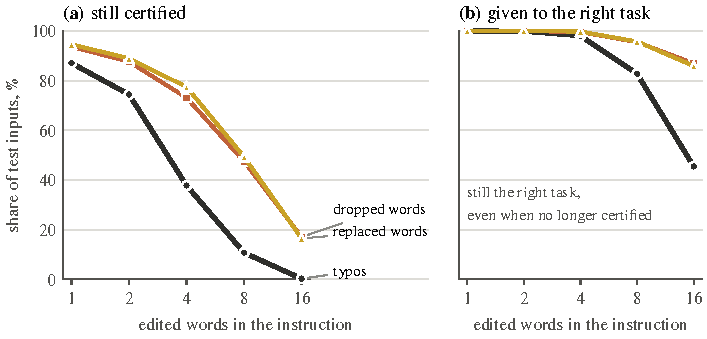
\includegraphics[width=0.86\linewidth]{figures/edits}
  \caption{Mechanical edits, fifteen tasks, routes only (1{,}197 inputs per point). (a) Inputs still
  inside their own zone. (b) Inputs given to their own task. No edited input was in a foreign zone.}
  \label{fig:edits}
\end{figure}

\begin{table}[t]
  \caption{Edits of the whole instruction (same test as Figure~\ref{fig:edits}). Tasks whose
  definition has a single sentence are left out of the last three rows.}
  \label{tab:edits}
  \centering
  \small
  \begin{tabular}{lccccc}
    \toprule
    Edit of the instruction & Tasks & Inputs & Certified inputs, \% & \shortstack[c]{Sent to own\\task, \% $\uparrow$} & Wrong zone \\
    \midrule
    Lower case & 15 & 1197 & 91.4 & 100.0 & 0 \\
    Sentence in front & 15 & 1197 & 91.6 & 100.0 & 0 \\
    First sentence removed & 14 & 1097 & 24.7 & 100.0 & 0 \\
    Last sentence removed & 14 & 1097 & 32.8 & 81.5 & 0 \\
    Sentences shuffled & 14 & 1097 & 100.0 & 100.0 & 0 \\
    \bottomrule
\end{tabular}

\end{table}

\paragraph{No edited input was certified for another task.} Not one of the 23{,}640 edited inputs
lay inside the zone of another task. An edited input was either certified for its own task or not
certified at all. This is a statement about these fifteen tasks, whose instructions are far apart;
in the large collection of Section~\ref{sec:many} the inputs of sibling tasks do lie inside older
zones. A certificate promises that an answer will stay the same, not that it comes from the right
task.

\paragraph{Small edits keep the certificate, large ones lose it.} With one typo 87.1\% of the inputs
are still certified, with one dropped word 93.7\%, with one replaced word 94.6\%, in lower case
91.4\% and with a sentence in front 91.6\% (Figure~\ref{fig:edits}a,
Table~\ref{tab:edits}). With four edited words between 38\% and 77\% remain certified, with sixteen
at most 17\%. A typo costs more than a dropped word, presumably because a misspelt word falls apart into
several rare word pieces, which carry a high weight in Eq.~\eqref{eq:weights}.

\paragraph{The route of an uncertified input is not safe under heavy damage.} Up to four edited
words, at least 98.1\% of the inputs still reach their own task. With eight typos it is 82.7\%, and
with sixteen typos only 45.4\% (Figure~\ref{fig:edits}b). Before the test we had written down that a
share under 80\% for any edit would count against the method, and it does: when an instruction is
badly damaged, the nearest-zone route cannot be relied on. What the method offers in this situation
is the missing certificate, which marks every one of these inputs.

\paragraph{Long instructions are robust, short ones are not.} The failures are not spread evenly
(Table~\ref{tab:editspertask} in the appendix). Tasks whose opening has at least 90 tokens keep
98\% to 100\% of their inputs on the right task even with sixteen typos. The two tasks that fail
first have the shortest instructions: \texttt{sciq}, whose definition has ten words (opening of 26
tokens), and \texttt{xsum} (34 tokens); with eight typos only 3\% and 18\% of their inputs arrive.
With sixteen typos every word of four or more letters in a definition of ten words carries a typo.

\paragraph{Two findings that follow from how the switch reads.} Removing the last sentence of the
definition leaves 81.5\% of the inputs on their task, but only 2\% for SST-2 and 8\% for emotion
classification: in both, the removed sentence is the one that states the task. Shuffling the
sentences changes nothing at all, and every input stays certified, because the feature of
Eq.~\eqref{eq:prefix} is an average and ignores the order of the words
(Proposition~\ref{prop:edits}).

\paragraph{The guaranteed tolerance.} The largest distance between two rows of the rescaled
embedding table of T5-base is $D = 509.6$, and the ratio $R_k / D$ of Proposition~\ref{prop:edits}
lies between 2.0\% and 4.2\% for the fifteen tasks. Edits that remove at most this share of the
weight of the opening, and add at most this share, can therefore never leave the zone. Counted in
tokens of average weight this is the replacement of \BoundTokensLow{} to \BoundTokensHigh{} tokens,
depending on the task. The measured tolerance is far larger, as it should be: the bound has to
cover the two most different tokens of the vocabulary. We also
checked the bound itself on \BoundInputs{} edited inputs of this test (ten per task and edit with
typos, dropped and replaced words). It held for every one of them; the inputs moved by at most
\BoundWorstPct{}\% of what the bound allows, \BoundMedianPct{}\% in the middle, and the bound
alone would have certified \BoundGuaranteed{} of the \BoundInside{} inputs that in fact stayed inside
their zone.


\subsection{The order of the tasks}
\label{sec:orders}

The signature of a task depends on its own opening only, and its radius on the signatures known
when the task arrives. How the routes would look if the tasks had arrived in another order can
therefore be computed exactly, without training. Table~\ref{tab:orders} does this for every one of
the 120 orders of the five tasks, and for the two official orders of the benchmark and 1{,}000 random
orders of the fifteen tasks.

\begin{table}[t]
  \caption{The order of the tasks (routes only, T5-base word-vectors). Entries with four numbers are
  for the original / light / medium / heavy wording; the reworded inputs are those of the five tasks.
  ``Blocked'': training inputs inside an older zone. ``Changed'': test inputs whose route changed
  after their task had been added; where a range is given it depends on the order.}
  \label{tab:orders}
  \centering
  \footnotesize
  \setlength{\tabcolsep}{3.5pt}
  \begin{tabular}{lcccccc}
    \toprule
    Sequence & Orders & \shortstack[c]{Sent to own\\task, \% $\uparrow$} & \shortstack[c]{Certified\\inputs, \%} & Wrong zone & Blocked & \shortstack[c]{Routes\\changed $\downarrow$} \\
    \midrule
    5 tasks, all orders & 120 & 100/100/100/93.8 & 100/100/20/19.6 & 0 & 0 & 0--31 \\
    \midrule
    15 tasks, official order 1 & 1 & 100/100/100/93.8 & 100/100/20/19.6 & 0 & 0 & 0 \\
    15 tasks, official order 2 & 1 & 100/100/100/93.8 & 100/100/20/19.6 & 0 & 0 & 31 \\
    15 tasks, random orders & 1,000 & 100/100/100/93.8 & 100/100/20/19.6 & 0 & 0 & 0--31 \\
    \bottomrule
\end{tabular}

\end{table}

In every order all inputs with the original wording are certified, no input lies in a foreign
zone, no training input is blocked, and the shares of inputs that reach their own task are the
same to the last digit. The reason is plain once the distances are written down
(Table~\ref{tab:distances} in the appendix). For 13 of the 15 tasks the nearest known signature is
that of an unrelated task, and the unrelated tasks are known from the start, so the radius of
these zones does not depend on the order at all. The two exceptions are the summarisation tasks
\texttt{samsum} and \texttt{xsum}, whose nearest signature is a third summarisation task
(\texttt{reddit\_tifu}); their radius is up to 7\% and 13\% smaller if that task was learned
before them, and no test input is affected.

What does depend on the order is \emph{when} an uncertified input goes wrong. The 31 heavily
reworded tweets that are given to SST-2 are given to it from the start if SST-2 is learned before
Sentiment140, as in our five-task sequence and in official order~1. If SST-2 comes later, as in
official order~2, they are first given to their own task and are re-routed at the moment SST-2
arrives. In that order 31 routes change after the inputs were first answered, and with a route the answer
changes in general (this test computes routes only). They are uncertified inputs, and
Proposition~\ref{prop:uncertified} says that this can happen; for certified ones it cannot.


\subsection{The unrelated inputs}
\label{sec:background}

The switch uses the collection $\mathcal{B}$ of unrelated inputs in three places: the token
weights, the scale of distances, and the signatures of the unrelated tasks, which set most radii.
A reader may ask whether the results depend on this particular collection. We repeated the route
computations with two other random draws of the 4{,}000 inputs, with 500, 1{,}000 and 2{,}000 inputs,
and with only five of the ten unrelated tasks, in two ways (Table~\ref{tab:background} in the
appendix; the settings and what would count against the method were again fixed beforehand). In
all eight settings every input with the original or the light wording is certified, every input
with the original, light or medium wording reaches its own task, no input lies in a foreign zone,
and no training input is blocked. The part of the results that rests on the guarantee therefore
did not depend on the choice. The share of heavily reworded inputs that reach their own task did:
it ranges from \BackgroundHeavyLow{}\% to \BackgroundHeavyHigh{}\% across the settings, so the value
of our main configuration, 93.8\%, is one draw from that range and not a property of the method.
One thing we had expected did not happen: with only five unrelated tasks the radii hardly changed (Table~\ref{tab:background}),
and at most two more heavily reworded inputs were certified.


\subsection{Other models}
\label{app:models}

\paragraph{The routes with other embedding tables.} The switch needs nothing from a model except its
tokenizer and its embedding table, so where the test inputs would be routed can be computed for any
model without training it. Table~\ref{tab:models} does this for eight models of three kinds:
encoder-decoder models (T5 in three sizes \citep{raffel2020t5} and Flan-T5
\citep{chung2024flant5}), decoder-only models (GPT-2 \citep{radford2019gpt2}, SmolLM2
\citep{allal2025smollm2} and Qwen2.5 \citep{yang2024qwen25}) and an encoder (RoBERTa
\citep{liu2019roberta}), with embedding dimensions from 512 to 1024 and five different
vocabularies. Nothing was adjusted per model; the radius factor and the word weights are those of
Section~\ref{sec:method}. For every model, every test input with the original wording lies in its
own zone, in the five-task and in the 15-task sequence, no input lies in a foreign zone, and no
training input of a later task is blocked. With light rewording 99\% to 100\% of the inputs are
certified, and with medium rewording all inputs still reach their own task. Heavy rewording is
where the models differ: between 80\% and 99\% of those inputs reach their own task. Under heavy rewording the routes of three uncertified inputs changed when a later task arrived (two with Flan-T5, one with GPT-2); no certified route changed.

\begin{table}[t]
  \caption{Routes computed with the embedding tables of eight models (CPU, no training). Entries
  with four numbers are for the original / light / medium / heavy wording. ``Wrong zone'': inputs
  inside the zone of another task, over both sequences and all wordings. ``Changed'': inputs
  whose route changed after their task had been added. With the original wording every input of
  the 15-task sequence is certified for every model.}
  \label{tab:models}
  \centering
  \footnotesize
  \setlength{\tabcolsep}{3pt}
  \begin{tabular}{lcccccc}
    \toprule
    & & \multicolumn{2}{c}{Five tasks} & Fifteen tasks & & \\
    \cmidrule(lr){3-4} \cmidrule(lr){5-5}
    Embedding table of & \shortstack[c]{Embedding\\dimension\\$d$} & \shortstack[c]{certified\\inputs, \%} & \shortstack[c]{sent to\\own task,\\\% $\uparrow$} & \shortstack[c]{sent to\\own task,\\\% $\uparrow$} & Wrong zone & \shortstack[c]{Routes\\changed\\$\downarrow$} \\
    \midrule
    \texttt{t5-small} & 512 & 100/100/20/20 & 100/100/100/89 & 100/100/100/89 & 0 & 0 \\
    \texttt{t5-base} & 768 & 100/100/20/20 & 100/100/100/94 & 100/100/100/94 & 0 & 0 \\
    \texttt{t5-large} & 1024 & 100/100/20/19 & 100/100/100/83 & 100/100/100/83 & 0 & 0 \\
    \texttt{flan-t5-base} & 768 & 100/100/20/14 & 100/100/100/99 & 100/100/100/99 & 0 & 2 \\
    \texttt{gpt2} & 768 & 100/99/20/20 & 100/100/100/87 & 100/100/100/87 & 0 & 1 \\
    \texttt{SmolLM2-135M} & 576 & 100/99/20/20 & 100/100/100/82 & 100/100/100/82 & 0 & 0 \\
    \texttt{Qwen2.5-0.5B} & 896 & 100/99/20/20 & 100/100/100/80 & 100/100/100/80 & 0 & 0 \\
    \texttt{roberta-base} & 768 & 100/99/20/20 & 100/100/100/94 & 100/100/100/93 & 0 & 0 \\
    \bottomrule
\end{tabular}

\end{table}

\paragraph{Training other models with the stand-alone code.} To check that the method, and not
only its routes, carries over to other models, we ran the stand-alone implementation
(Appendix~\ref{app:impl}) on three small models on a CPU: T5-small (encoder-decoder), GPT-2 and
SmolLM2-135M (both decoder-only). The runs are small on purpose: the five tasks with 400 training
examples and five epochs each, 30 to 50 test inputs per task, one seed. They show whether the code
keeps answers on another architecture, not how good these models can become. In all three runs
(Table~\ref{tab:demo}) the certified switch ends exactly where it stood right after learning, no
answer of an earlier task changes, and every test input with the original wording is certified. With
all adapters on, the same adapters end at \DemoTfivePlainAP{}, \DemoGptPlainAP{} and
\DemoSmolPlainAP{} instead of \DemoTfiveAP{}, \DemoGptAP{} and \DemoSmolAP{}, and nearly all answers of
earlier tasks change. With heavily reworded instructions no answer changes either, and
\DemoTfiveHeavyRight{}\%, \DemoGptHeavyRight{}\% and \DemoSmolHeavyRight{}\% of those inputs reach
their own task.

\begin{table}[t]
  \caption{The stand-alone implementation on three small models (CPU, five tasks, 400 training
  examples and 5 epochs per task, one seed). ``Changed'': answers of the first four tasks that
  differ at the end. ``Certified'': test inputs with the original wording that are inside a zone.
  ``enc.-dec.'': encoder-decoder; ``dec.-only'': decoder-only.}
  \label{tab:demo}
  \centering
  \footnotesize
  \setlength{\tabcolsep}{3pt}
  \begin{tabular}{llcccccccc}
    \toprule
    & & \multicolumn{3}{c}{\cert{}, original} & \multicolumn{2}{c}{\plain{}, original} & & \multicolumn{2}{c}{\cert{}, heavy} \\
    \cmidrule(lr){3-5} \cmidrule(lr){6-7} \cmidrule(lr){9-10}
    Model & Kind & \shortstack[c]{Score\\right\\after\\learning\\$\uparrow$} & \shortstack[c]{Final\\score\\$\uparrow$} & \shortstack[c]{Answers\\changed $\downarrow$} & \shortstack[c]{Final\\score\\$\uparrow$} & \shortstack[c]{Answers\\changed $\downarrow$} & \shortstack[c]{Certified\\inputs} & \shortstack[c]{Final\\score\\$\uparrow$} & \shortstack[c]{Answers\\changed $\downarrow$} \\
    \midrule
    \texttt{SmolLM2-135M} & dec.-only & 74.3 & 74.3 & 0 of 120 & 27.7 & 100 of 120 & 150 of 150 & 65.1 & 0 of 120 \\
    \texttt{gpt2} & dec.-only & 67.9 & 67.9 & 0 of 120 & 15.8 & 119 of 120 & 150 of 150 & 54.8 & 0 of 120 \\
    \texttt{t5-small} & enc.-dec. & 65.8 & 65.8 & 0 of 200 & 12.0 & 200 of 200 & 250 of 250 & 56.2 & 0 of 200 \\
    \bottomrule
\end{tabular}

\end{table}

\paragraph{A sibling task, with trained answers.} The variant \exactfirst{} was also run with the
stand-alone code on T5-small. After the five tasks a sixth task is learned: the sentences of SST-2
under the lightly reworded definition of SST-2, but with other answer words (``good'' and ``bad''
instead of ``POS'' and ``NEG''), so that one can see which adapters answered. The sixth task is
learned twice from the same starting point. Under \cert{}, all \SiblingCertBlocked{} of its
\SiblingTrain{} training inputs are blocked; after training, its test inputs are still answered in
the words of the old task (\SiblingCertRight{} of \SiblingTest{} right), and no answer of the five
old tasks changes in any wording. Under \exactfirst{} the task is learned (\SiblingExactRight{} of
\SiblingTest{} right), no answer to an unedited input of the old tasks changes, and the
\SiblingExactChangedLight{} old test inputs of SST-2 that carry the sibling's instruction word for
word now get the sibling's answer; nothing else changes (\SiblingOldInputs{} old test inputs per
wording). This is one small model and one constructed sibling. It shows the two behaviours side by
side with trained answers, and it is not a test of the variant at scale.



